\documentclass{article}
\usepackage{graphicx}
\usepackage{tikz}

\begin{document}
\begin{figure}[h]
  \centering
  \begin{minipage}[b]{0.45\textwidth}
    \centering
    \fbox{
      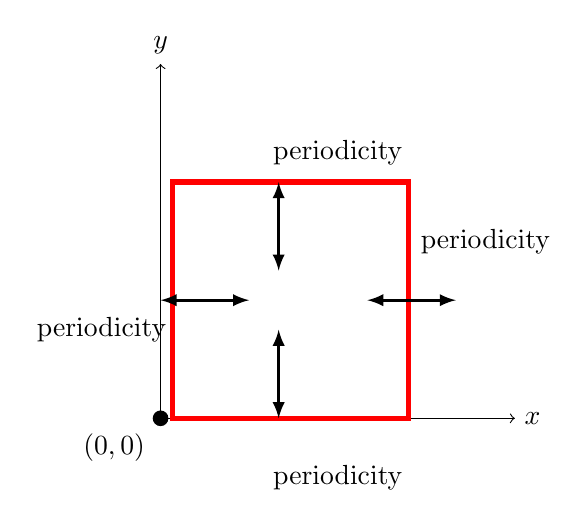
\begin{tikzpicture}[scale=1.5]
        % 绘制坐标轴
        \draw[->] (0,0) -- (3,0) node[right] {$x$};
        \draw[->] (0,0) -- (0,3) node[above] {$y$};
        % 标注原点和轴名称
        \node[circle,fill,inner sep=2pt,label=below left:{$(0,0)$}] at (0,0) {};

        % 绘制正方形
        \draw[red, line width=2pt] (0.1,0) rectangle (2.1,2);

        % 标注实心箭头和文字
        \draw[latex-latex, line width=1pt, fill=black] (0,1) -- (0.75,1);
        \node at (-0.5,0.75) {periodicity};

        \draw[latex-latex, line width=1pt, fill=black] (1,0) -- (1,0.75);
        \node at (1.5,-0.5) {periodicity};

        \draw[latex-latex, line width=1pt, fill=black] (1,2) -- (1,1.25);
        \node at (1.5,2.25) {periodicity};

        \draw[latex-latex, line width=1pt, fill=black] (2.5,1) -- (1.75,1);
        \node at (2.75,1.5) {periodicity};
      \end{tikzpicture}
    }
    \caption{Pic1}
    \label{img::left}
  \end{minipage}
  
  %\hfill%空隙
  
  \begin{minipage}[b]{0.45\textwidth}
    \centering
    \fbox{
      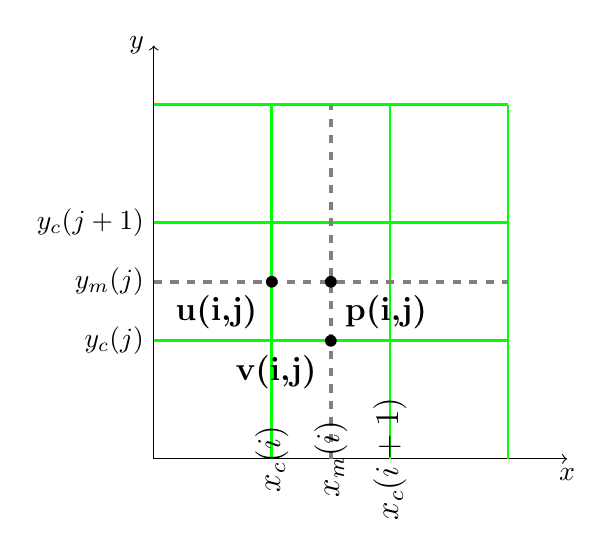
\begin{tikzpicture}[scale=1.5]
        % 绘制坐标轴
        \draw[->] (0,0) -- (3.5,0) node[below] {$x$};
        \draw[->] (0,0) -- (0,3.5) node[left] {$y$};

        % 绘制网格线
        \foreach \x in {1,2,3}
          \draw[green, line width=1pt] (\x,0) -- (\x,3);
        \foreach \y in {1,2,3}
          \draw[green, line width=1pt] (0,\y) -- (3,\y);

        % 绘制虚线
        \draw[dashed, gray, line width=1.5pt] (1.5,0) -- (1.5,3);
        \draw[dashed, gray, line width=1.5pt] (0,1.5) -- (3,1.5);

        % 标注点
        \node[circle,fill,inner sep=1.5pt,label={[font=\large\bfseries]below left:\textbf{u(i,j)}}] at (1,1.5) {};
        \node[circle,fill,inner sep=1.5pt,label={[font=\large\bfseries]below right:\textbf{p(i,j)}}] at (1.5,1.5) {};
        \node[circle,fill,inner sep=1.5pt,label={[font=\large\bfseries]below left:\textbf{v(i,j)}}] at (1.5,1) {};

        % 标注刻度
        \node[rotate=90, font=\large] at (1,0) {$x_c(i)$};
	\node[rotate=90, font=\large] at (1.5,0) {$x_m(i)$};
	\node[rotate=90, font=\large] at (2,0) {$x_c(i+1)$};

        \node[left] at (0,1) {$y_c(j)$};
        \node[left] at (0,1.5) {$y_m(j)$};
        \node[left] at (0,2) {$y_c(j+1)$};
      \end{tikzpicture}
    }
    \caption{Pic2}
    \label{img::right}
  \end{minipage}
\end{figure}


adfasdfasdfsdaf\ref{img::left}FFFFFFFfasdfasdfa
\end{document}

